\chapter{Prompty systemu}\label{app:prompty}

Dodatek zawiera moduł \texttt{sources/config/prompts.py} z~promptami
wykorzystywanymi w~systemie. Ich wydzielenie zwiększa czytelność opisu
implementacji w~rozdziale~\ref{chap:implementacja} i~umożliwia weryfikację
treści instrukcji przekazywanych modelom.

\lstdefinestyle{promptlisting}{
  language=Python,
  basicstyle=\ttfamily\tiny,
  breaklines=true,
  breakatwhitespace=true,
  columns=fullflexible,
  keepspaces=true,
  showstringspaces=false,
  literate=
  {ą}{{\k{a}}}1 {ę}{{\k{e}}}1 {ó}{{\'o}}1 {ś}{{\'s}}1
  {ł}{{\l{}}}1 {ż}{{\.z}}1 {ź}{{\'z}}1 {ć}{{\'c}}1 {ń}{{\'n}}1
  {Ą}{{\k{A}}}1 {Ę}{{\k{E}}}1 {Ó}{{\'O}}1 {Ś}{{\'S}}1
  {Ł}{{\L{}}}1 {Ż}{{\.Z}}1 {Ź}{{\'Z}}1 {Ć}{{\'C}}1 {Ń}{{\'N}}1
  {§}{{\S{}}}1 {—}{{--}}1
  {✓}{{\checkmark}}1 {✗}{{\(\times\)}}1,
}

Prompt \texttt{EXTRACTION\_PROMPT} służy jako instrukcja systemowa dla modelu
multimodalnego podczas ekstrakcji tekstu ze stron dokumentów ubezpieczeniowych
metodą OCR.

\lstinputlisting[
  style=promptlisting,
  firstline=13,
  lastline=45,
  caption={Prompt ekstrakcji tekstu OCR (\texttt{EXTRACTION\_PROMPT})},
  label={lst:app-extraction-prompt}
]{../code/sources/config/prompts.py}

Prompt \texttt{QUESTION\_PARSER\_SYSTEM\_PROMPT} definiuje proces wyodrębniania
strukturalnych metadanych z~pytania użytkownika na potrzeby filtrowania w~bazie
wektorowej Qdrant.

\lstinputlisting[
  style=promptlisting,
  firstline=47,
  lastline=96,
  caption={Prompt parsera pytań (\texttt{QUESTION\_PARSER\_SYSTEM\_PROMPT})},
  label={lst:app-question-parser-prompt}
]{../code/sources/config/prompts.py}

Prompt \texttt{QUERY\_REWRITER\_SYSTEM\_PROMPT} służy do generowania trzech
zróżnicowanych leksykalnie wariantów zapytania na potrzeby wyszukiwania
wektorowego.

\lstinputlisting[
  style=promptlisting,
  firstline=98,
  lastline=117,
  caption={Prompt przepisania zapytań (\texttt{QUERY\_REWRITER\_SYSTEM\_PROMPT})},
  label={lst:app-query-rewriter-prompt}
]{../code/sources/config/prompts.py}

Prompt \texttt{RERANKER\_SYSTEM\_PROMPT} definiuje kryteria dla modelu
oceniającego trafność każdego pobranego fragmentu dokumentu względem zadanego
pytania w~skali 0--1.

\lstinputlisting[
  style=promptlisting,
  firstline=119,
  lastline=140,
  caption={Prompt oceny trafności fragmentów (\texttt{RERANKER\_SYSTEM\_PROMPT})},
  label={lst:app-reranker-prompt}
]{../code/sources/config/prompts.py}

Prompt \texttt{REFERENCE\_CORRECTNESS\_PROMPT} jest wykorzystywany przez
ewaluator Phoenix do oceny poprawności wygenerowanej odpowiedzi względem
wzorcowej odpowiedzi referencyjnej.

\lstinputlisting[
  style=promptlisting,
  firstline=142,
  lastline=175,
  caption={Prompt oceny poprawności odpowiedzi (\texttt{REFERENCE\_CORRECTNESS\_PROMPT})},
  label={lst:app-reference-correctness-prompt}
]{../code/sources/config/prompts.py}

Prompt \texttt{CONCISENESS\_PROMPT} jest używany przez ewaluator Phoenix do
oceny zwięzłości odpowiedzi generowanej przez system.

\lstinputlisting[
  style=promptlisting,
  firstline=177,
  lastline=210,
  caption={Prompt oceny zwięzłości odpowiedzi (\texttt{CONCISENESS\_PROMPT})},
  label={lst:app-conciseness-prompt}
]{../code/sources/config/prompts.py}

Prompt \texttt{PLANNER\_SYSTEM\_PROMPT} definiuje zadanie agenta planisty
polegające na opracowaniu optymalnego planu wywołań narzędzi dla danego pytania
użytkownika.

\lstinputlisting[
  style=promptlisting,
  firstline=212,
  lastline=235,
  caption={Prompt agenta planisty (\texttt{PLANNER\_SYSTEM\_PROMPT})},
  label={lst:app-planner-prompt}
]{../code/sources/config/prompts.py}

Prompt \texttt{REACT\_SYSTEM\_PROMPT} definiuje pętlę rozumowania i~działania
agenta ReAct, określając format kroków myślenia oraz reguły korzystania
z~narzędzi.

\lstinputlisting[
  style=promptlisting,
  firstline=237,
  lastline=270,
  caption={Prompt agenta ReAct (\texttt{REACT\_SYSTEM\_PROMPT})},
  label={lst:app-react-prompt}
]{../code/sources/config/prompts.py}

Prompt \texttt{ROUTER\_SYSTEM\_PROMPT} służy do klasyfikacji pytania
użytkownika do jednej z~ośmiu zdefiniowanych kategorii tematycznych.

\lstinputlisting[
  style=promptlisting,
  firstline=272,
  lastline=294,
  caption={Prompt klasyfikatora kategorii pytań (\texttt{ROUTER\_SYSTEM\_PROMPT})},
  label={lst:app-router-prompt}
]{../code/sources/config/prompts.py}

Prompt \texttt{DECOMPOSER\_SYSTEM\_PROMPT} określa zasady podziału złożonego
pytania użytkownika na maksymalnie trzy niezależne podpytania.

\lstinputlisting[
  style=promptlisting,
  firstline=296,
  lastline=307,
  caption={Prompt dekompozycji pytań (\texttt{DECOMPOSER\_SYSTEM\_PROMPT})},
  label={lst:app-decomposer-prompt}
]{../code/sources/config/prompts.py}

Prompt \texttt{MERGE\_ANSWERS\_SYSTEM\_PROMPT} definiuje zasady scalania
odpowiedzi cząstkowych na poszczególne podpytania w~jedną spójną odpowiedź
w~języku polskim.

\lstinputlisting[
  style=promptlisting,
  firstline=309,
  lastline=337,
  caption={Prompt scalania odpowiedzi cząstkowych (\texttt{MERGE\_ANSWERS\_SYSTEM\_PROMPT})},
  label={lst:app-merge-answers-prompt}
]{../code/sources/config/prompts.py}

Szablon \texttt{\_ANSWER\_FORMAT} definiuje obligatoryjną strukturę wyjścia
(sekcje \textbf{Odpowiedź} i~\textbf{Szczegóły}) oraz zbiór reguł dla
wszystkich promptów odpowiedzi domenowych.

\lstinputlisting[
  style=promptlisting,
  firstline=339,
  lastline=372,
  caption={Szablon formatu odpowiedzi (\texttt{\_ANSWER\_FORMAT})},
  label={lst:app-answer-format}
]{../code/sources/config/prompts.py}

Prompt \texttt{FAQ\_PROMPT} formułuje zasady udzielania zwięzłych
i~precyzyjnych odpowiedzi na pytania faktograficzne dotyczące dokumentów
ubezpieczeniowych.

\lstinputlisting[
  style=promptlisting,
  firstline=374,
  lastline=384,
  caption={Prompt odpowiedzi FAQ (\texttt{FAQ\_PROMPT})},
  label={lst:app-faq-prompt}
]{../code/sources/config/prompts.py}

Prompt \texttt{DESCRIPTION\_PROMPT} służy do generowania zwięzłego opisu
produktu lub zakresu ochrony na podstawie pobranych fragmentów kontekstu.

\lstinputlisting[
  style=promptlisting,
  firstline=386,
  lastline=395,
  caption={Prompt opisu produktu (\texttt{DESCRIPTION\_PROMPT})},
  label={lst:app-description-prompt}
]{../code/sources/config/prompts.py}

Prompt \texttt{CLAIMS\_PROMPT} definiuje wytyczne do opisu procedury zgłaszania
i~obsługi szkody, w~tym kroków, terminów i~wymaganych dokumentów.

\lstinputlisting[
  style=promptlisting,
  firstline=397,
  lastline=405,
  caption={Prompt obsługi szkód (\texttt{CLAIMS\_PROMPT})},
  label={lst:app-claims-prompt}
]{../code/sources/config/prompts.py}

Prompt \texttt{COMPARISON\_PROMPT} określa format zestawienia produktów,
wariantów lub firm ubezpieczeniowych w~postaci tabeli Markdown.

\lstinputlisting[
  style=promptlisting,
  firstline=407,
  lastline=418,
  caption={Prompt porównania produktów (\texttt{COMPARISON\_PROMPT})},
  label={lst:app-comparison-prompt}
]{../code/sources/config/prompts.py}

Prompt \texttt{ELIGIBILITY\_PROMPT} ustala zasady wyjaśniania kryteriów
uprawnienia do ochrony, rozróżniając warunki obowiązkowe, opcjonalne
i~wyłączenia podmiotowe.

\lstinputlisting[
  style=promptlisting,
  firstline=420,
  lastline=431,
  caption={Prompt warunków uprawnienia do ochrony (\texttt{ELIGIBILITY\_PROMPT})},
  label={lst:app-eligibility-prompt}
]{../code/sources/config/prompts.py}

Prompt \texttt{PRICING\_PROMPT} określa sposób prezentacji informacji cenowych
i~finansowych z~dokumentów polisowych, takich jak sumy ubezpieczenia czy
składki.

\lstinputlisting[
  style=promptlisting,
  firstline=433,
  lastline=445,
  caption={Prompt informacji cenowych (\texttt{PRICING\_PROMPT})},
  label={lst:app-pricing-prompt}
]{../code/sources/config/prompts.py}

Prompt \texttt{COVERAGE\_PROMPT} wymusza sformułowanie jednoznacznego werdyktu
(Tak/Nie/Warunkowo) w~kwestii objęcia danego zdarzenia ochroną ubezpieczeniową.

\lstinputlisting[
  style=promptlisting,
  firstline=447,
  lastline=464,
  caption={Prompt zakresu ochrony (\texttt{COVERAGE\_PROMPT})},
  label={lst:app-coverage-prompt}
]{../code/sources/config/prompts.py}

Prompt \texttt{CONDITIONS\_PROMPT} określa wytyczne do wyjaśniania warunków
umownych, obowiązków ubezpieczonego i~wymagań formalnych wynikających
z~dokumentów OWU.

\lstinputlisting[
  style=promptlisting,
  firstline=466,
  lastline=479,
  caption={Prompt warunków umowy (\texttt{CONDITIONS\_PROMPT})},
  label={lst:app-conditions-prompt}
]{../code/sources/config/prompts.py}

Prompt \texttt{LIMITS\_PROMPT} definiuje zasady precyzyjnego przytaczania
limitów świadczeń, sum ubezpieczenia i~franszyz z~podaniem odniesień do
konkretnych klauzul OWU.

\lstinputlisting[
  style=promptlisting,
  firstline=481,
  lastline=498,
  caption={Prompt limitów i sum ubezpieczenia (\texttt{LIMITS\_PROMPT})},
  label={lst:app-limits-prompt}
]{../code/sources/config/prompts.py}

Prompt \texttt{EXCLUSIONS\_PROMPT} definiuje schemat kategoryzacji i~wyliczania
wyłączeń odpowiedzialności, grupując je na ogólne, przedmiotowe, podmiotowe
i~warunkowe.

\lstinputlisting[
  style=promptlisting,
  firstline=500,
  lastline=517,
  caption={Prompt wyłączeń ubezpieczenia (\texttt{EXCLUSIONS\_PROMPT})},
  label={lst:app-exclusions-prompt}
]{../code/sources/config/prompts.py}

Stała \texttt{CONTEXT\_INSTRUCTION} jest dołączana do każdego zapytania
syntezatora odpowiedzi jako przypomnienie reguł formatowania i~korzystania
wyłącznie z~pobranego kontekstu.

\lstinputlisting[
  style=promptlisting,
  firstline=519,
  lastline=533,
  caption={Instrukcja kontekstu dla syntezatora (\texttt{CONTEXT\_INSTRUCTION})},
  label={lst:app-context-instruction}
]{../code/sources/config/prompts.py}

\chapter{Diagramy architektur agentowych}\label{app:diagramy}

Dodatek zawiera diagramy sześciu architektur agentowych zaimplementowanych
w~module \texttt{sources/agents}. Diagramy zostały wygenerowane automatycznie
z~definicji \texttt{Mermaid} przez \texttt{utilities/drawer.py} i~zrenderowane
do plików PDF poleceniem \texttt{mmdc} z~opcją \texttt{-{}-pdfFit}.

\begin{figure}[H]
  \caption{Architektura deterministyczna}\label{fig:graf-architektury-deterministycznej}
  \centering
  \begin{adjustbox}{max width=0.85\textwidth,
    max totalheight=0.82\textheight, keepaspectratio}
    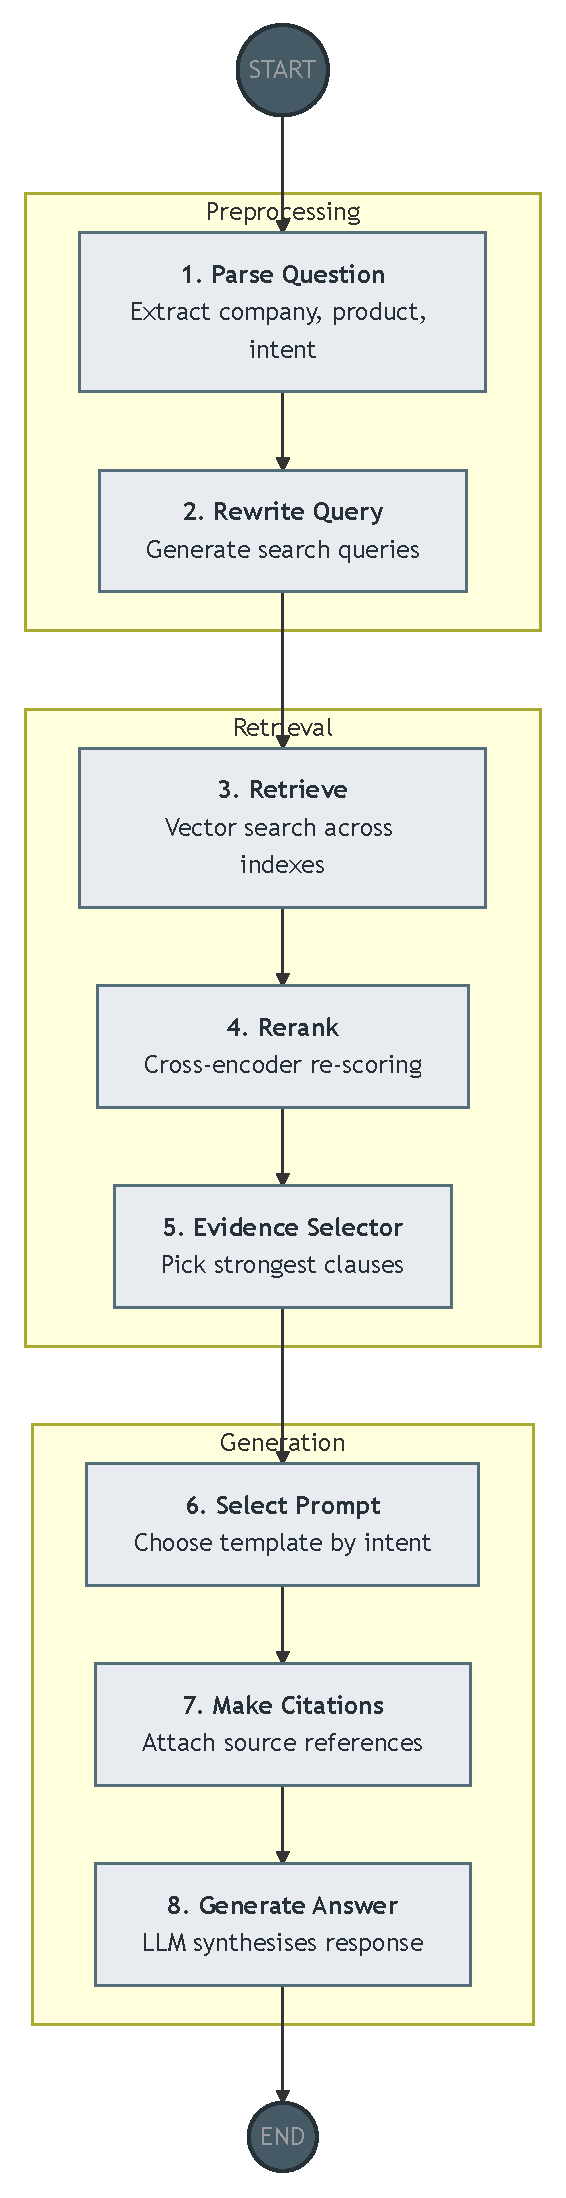
\includegraphics{../code/data/diagrams/deterministic.pdf}
  \end{adjustbox}
  \zrodlo{opracowanie własne}
\end{figure}

\begin{figure}[H]
  \caption{Architektura planer--wykonawca}\label{fig:graf-architektury-planer-wykonawca}
  \centering
  \begin{adjustbox}{max width=0.85\textwidth,
    max totalheight=0.82\textheight, keepaspectratio}
    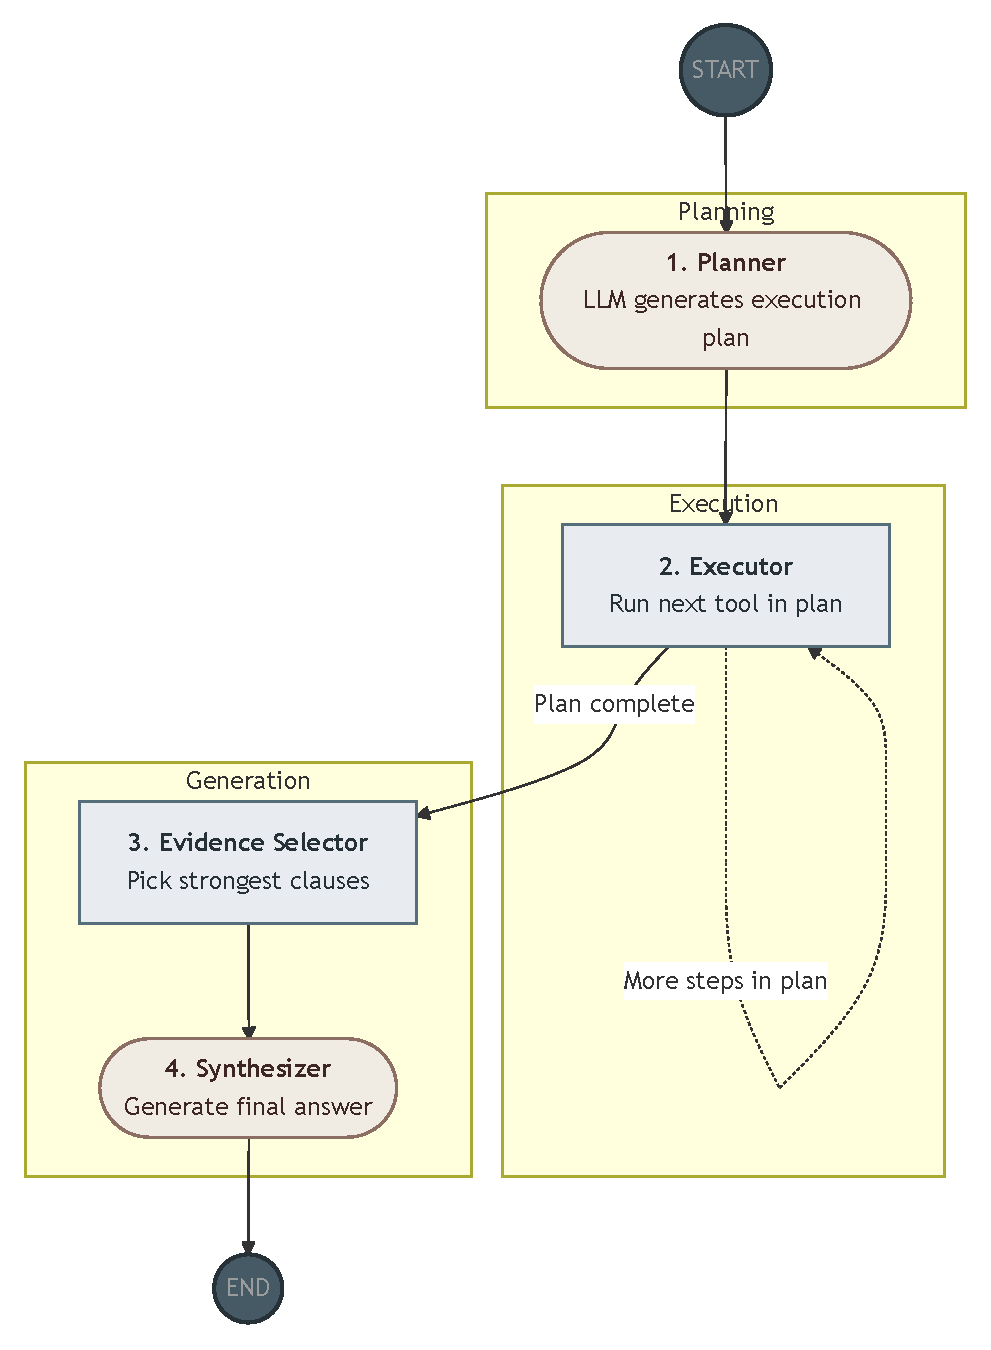
\includegraphics{../code/data/diagrams/planner_executor.pdf}
  \end{adjustbox}
  \zrodlo{opracowanie własne}
\end{figure}

\begin{figure}[H]
  \caption{Architektura router--specjalista}\label{fig:graf-architektury-router-specjalista}
  \centering
  \begin{adjustbox}{max width=0.85\textwidth,
    max totalheight=0.82\textheight, keepaspectratio}
    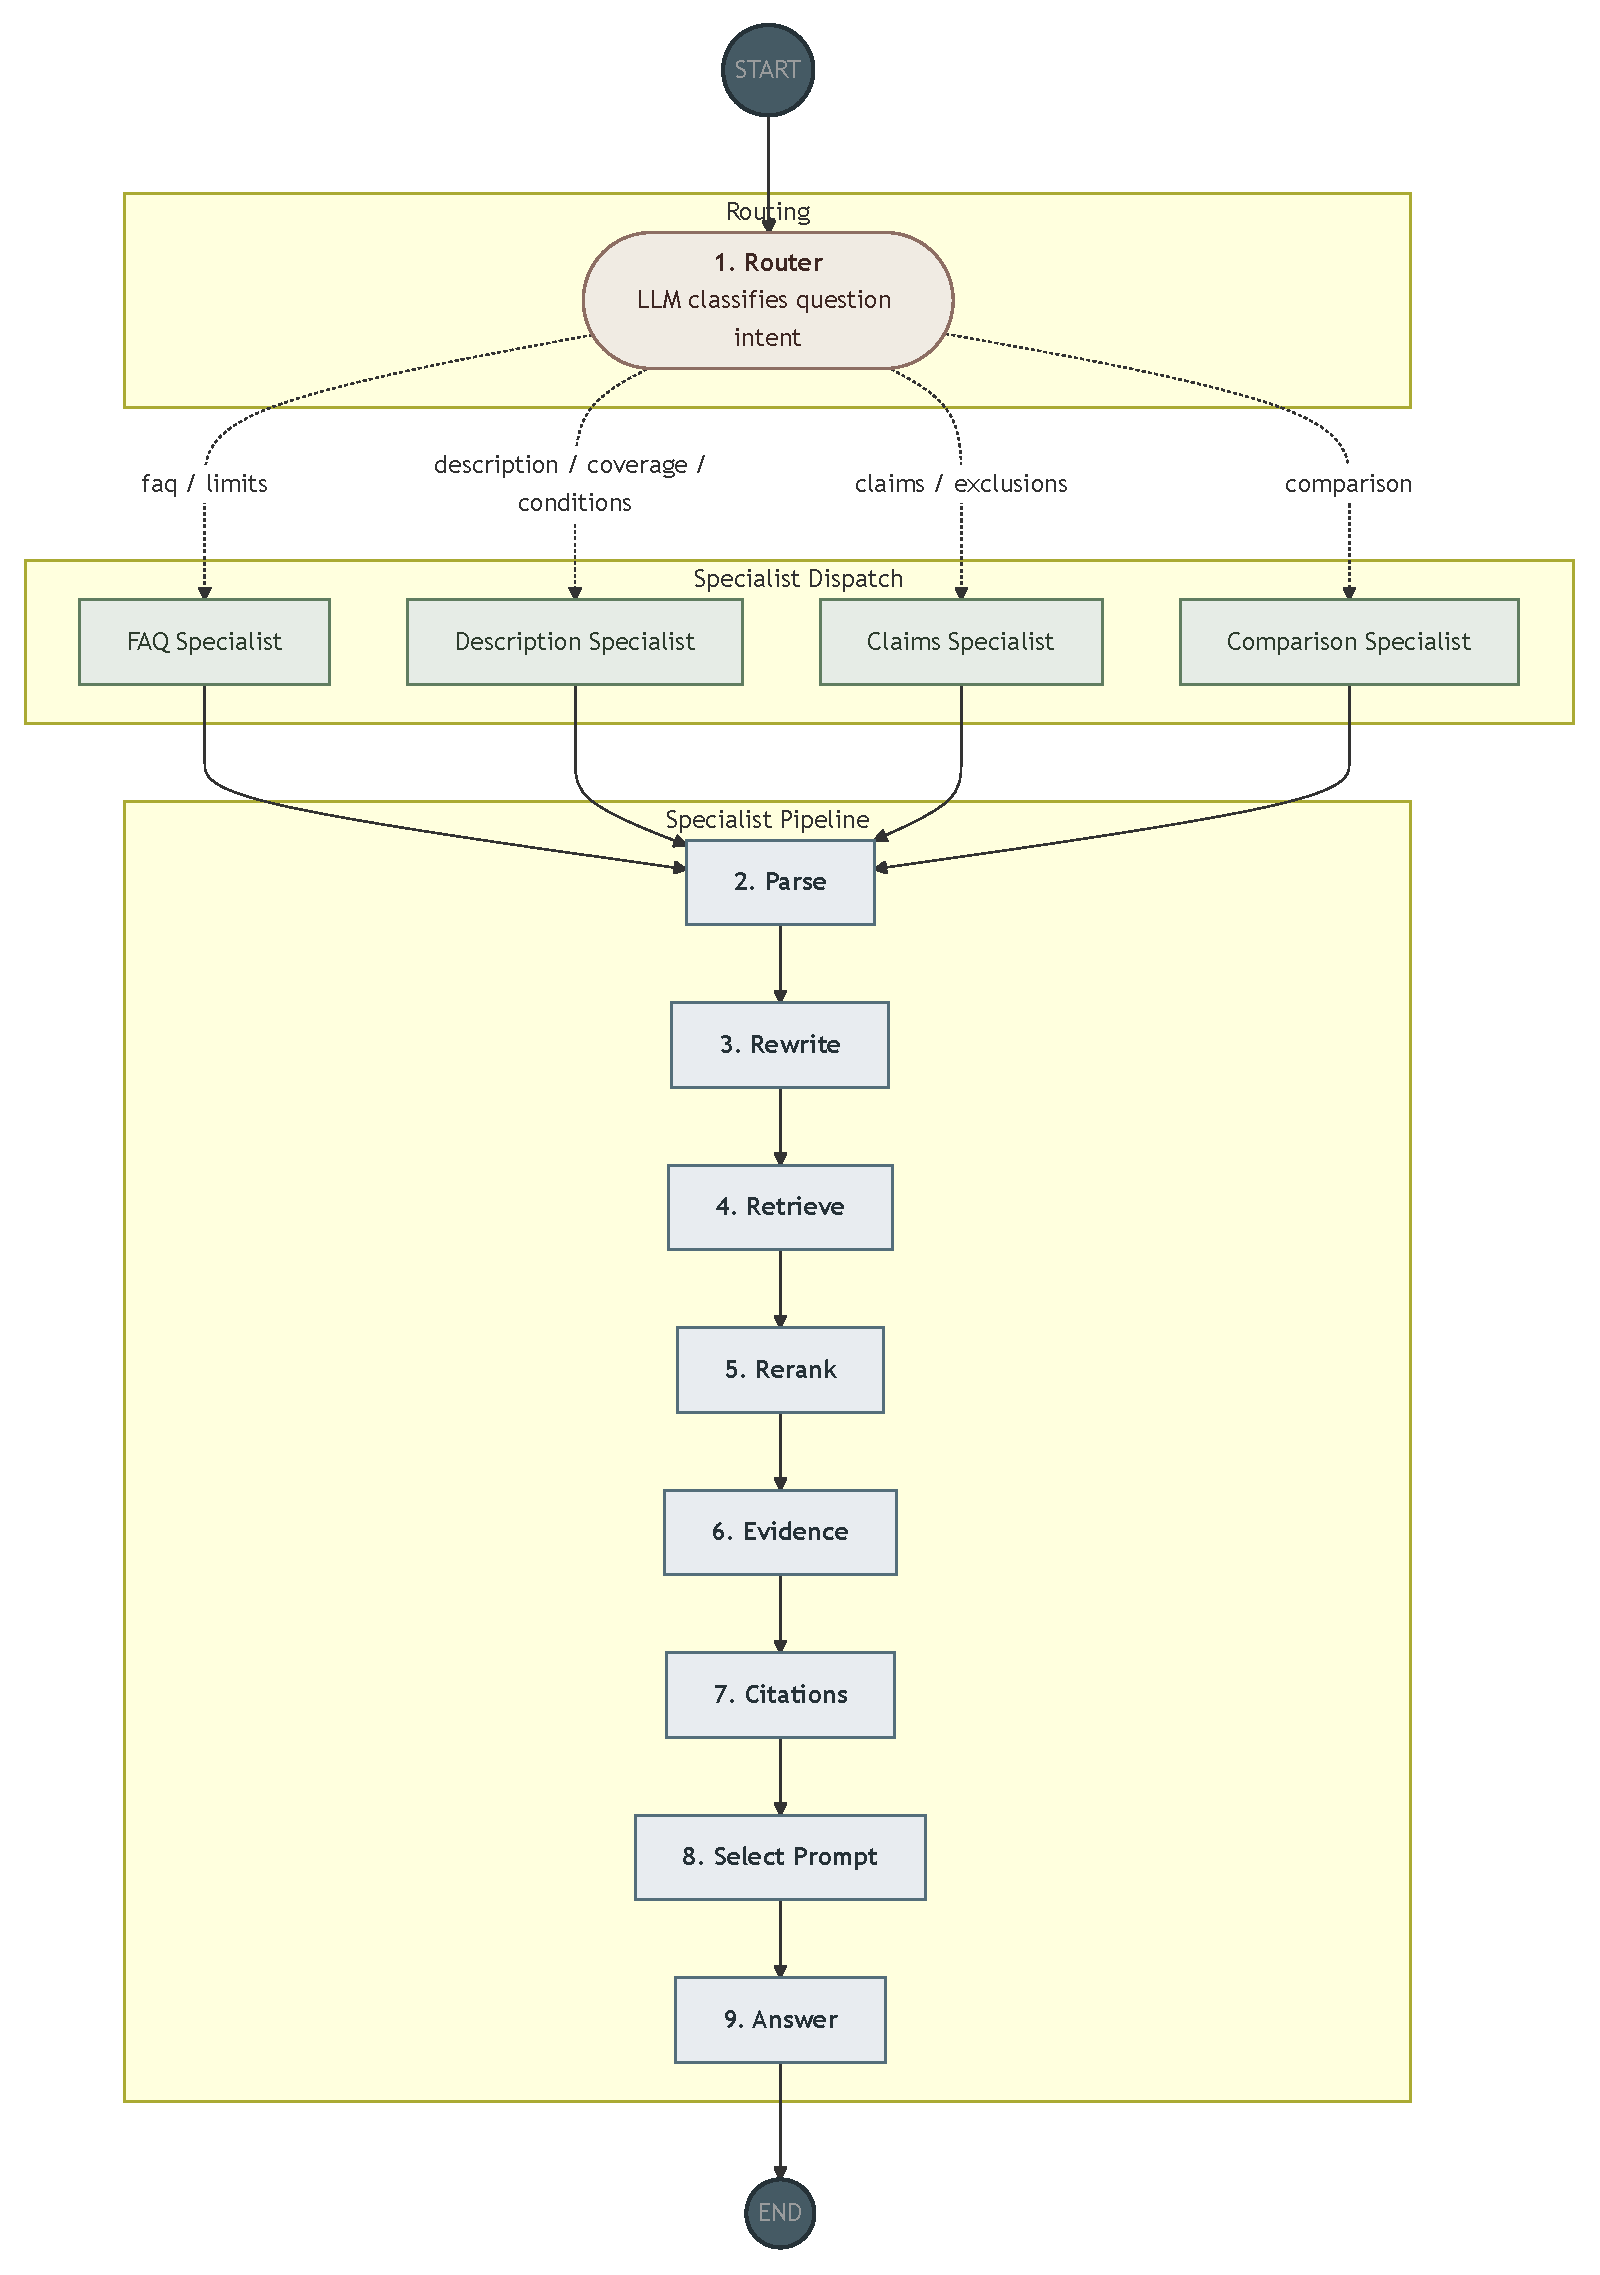
\includegraphics{../code/data/diagrams/router_specialist.pdf}
  \end{adjustbox}
  \zrodlo{opracowanie własne}
\end{figure}

\begin{figure}[H]
  \caption{Architektura tablicowa}\label{fig:graf-architektury-tablicowej}
  \centering
  \begin{adjustbox}{max width=0.85\textwidth,
    max totalheight=0.82\textheight, keepaspectratio}
    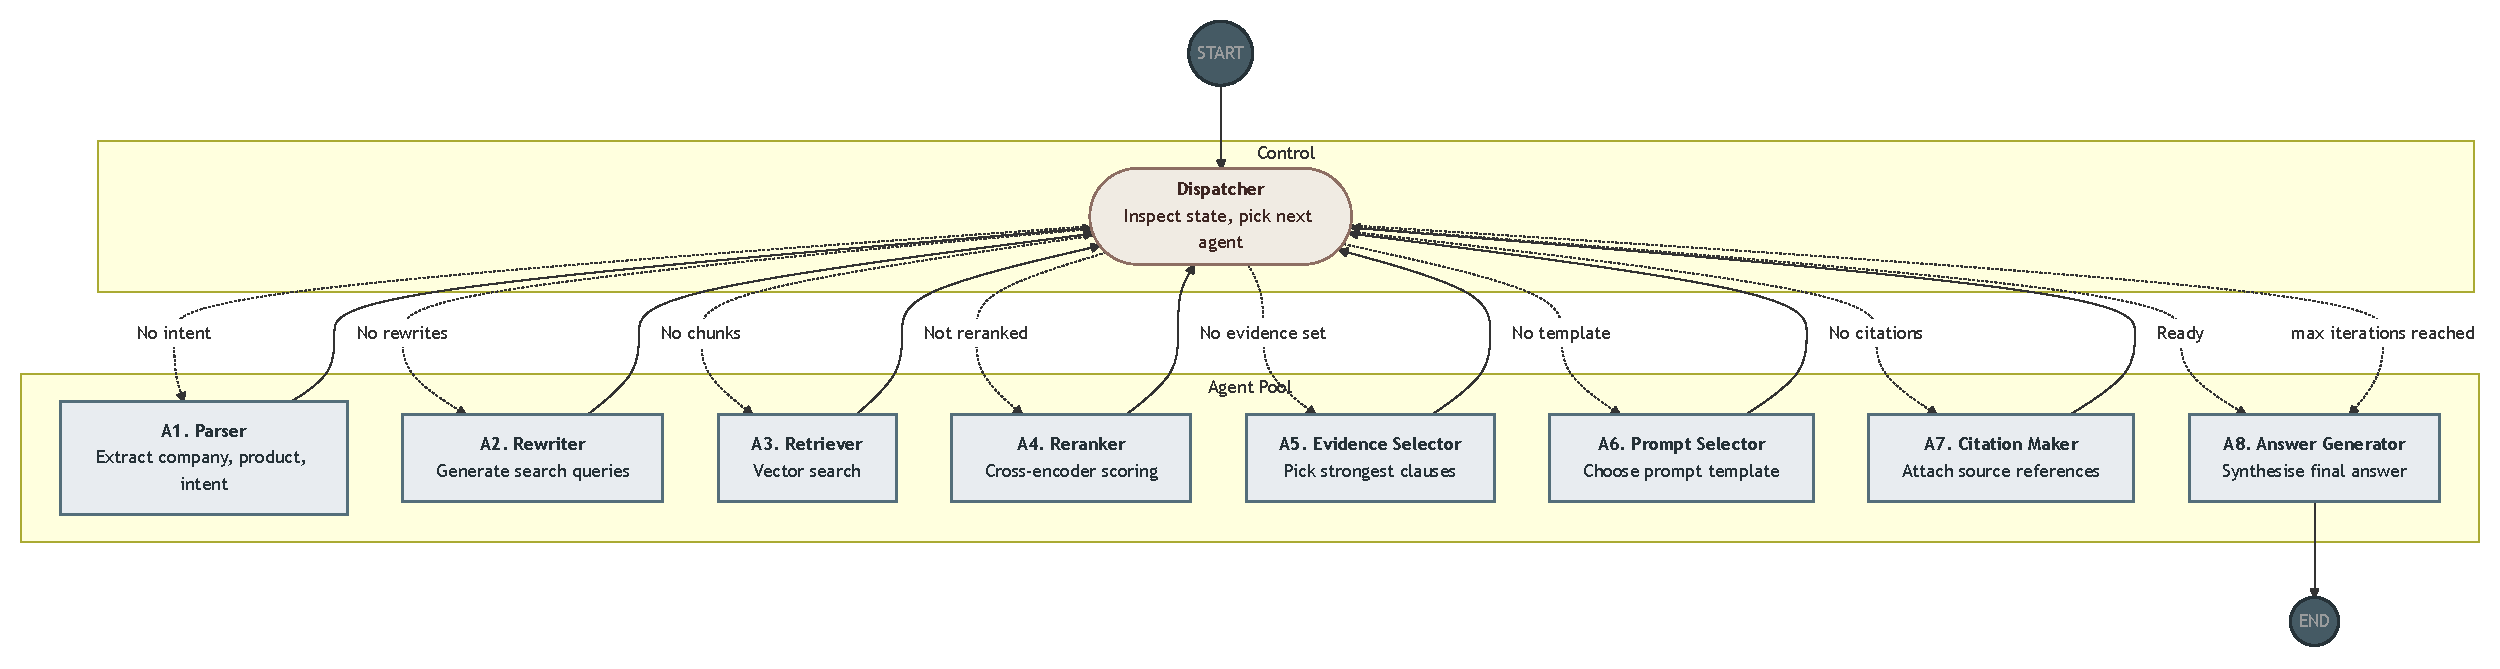
\includegraphics{../code/data/diagrams/blackboard.pdf}
  \end{adjustbox}
  \zrodlo{opracowanie własne}
\end{figure}

\begin{figure}[H]
  \caption{Architektura hierarchiczna}\label{fig:graf-architektury-hierarchicznej}
  \centering
  \begin{adjustbox}{max width=0.85\textwidth,
    max totalheight=0.82\textheight, keepaspectratio}
    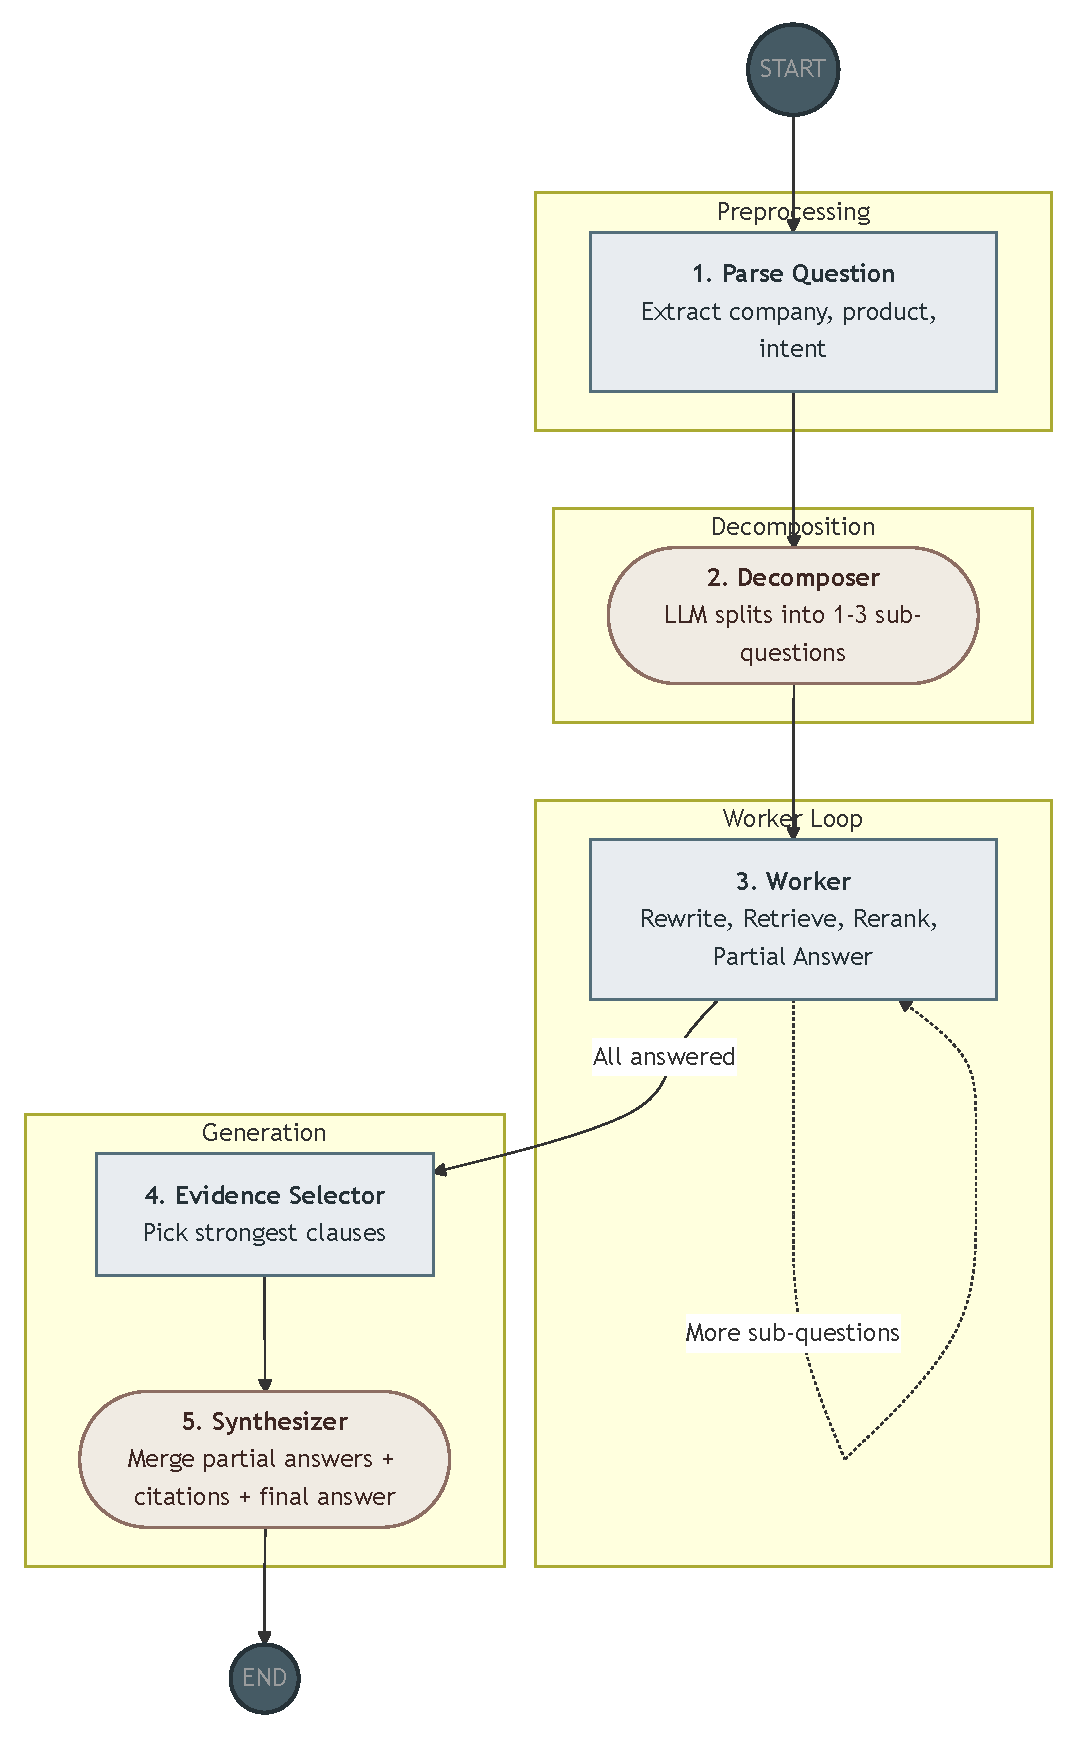
\includegraphics{../code/data/diagrams/hierarchical.pdf}
  \end{adjustbox}
  \zrodlo{opracowanie własne}
\end{figure}

\begin{figure}[H]
  \caption{Architektura ReAct}\label{fig:graf-architektury-react}
  \centering
  \begin{adjustbox}{max width=0.85\textwidth,
    max totalheight=0.82\textheight, keepaspectratio}
    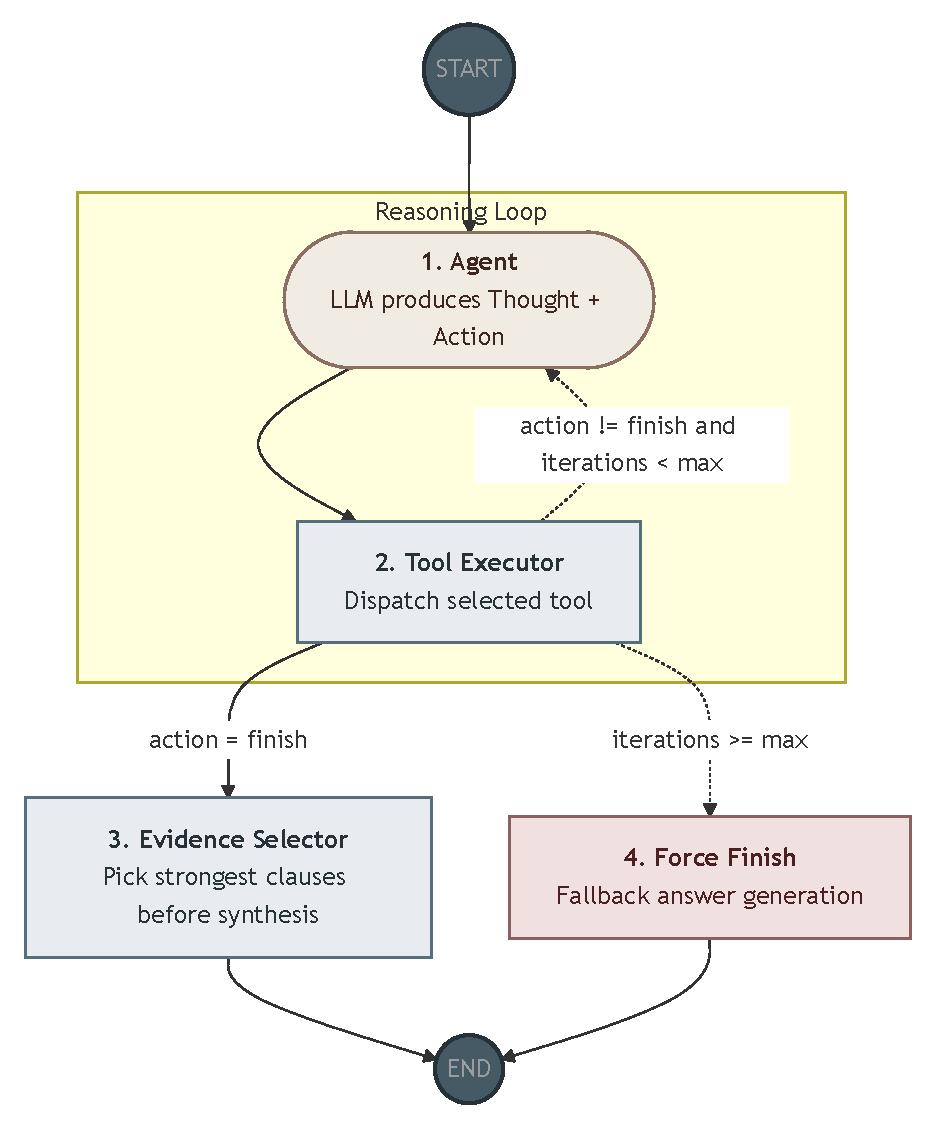
\includegraphics{../code/data/diagrams/react.pdf}
  \end{adjustbox}
  \zrodlo{opracowanie własne}
\end{figure}